% 两个原子间的相互作用
% 原子|散射问题|薛定谔方程

冷原子有他很独到的地方:
\begin{itemize}
\item 1. 很冷,所以粒子动能很低,我们只需要一个低能理论
\item 2. 相互作用很弱,很多时候都是 short-range ($\propto \E^{-kr}$) 的,有一个截止距离$r_0$
\item 3. 原子非常稀薄,可以暂时不使用多体理论,而是使用少体散射解决一定问题
\end{itemize}

在更深入的研究之前,我们先回顾一下两体散射过程的量子力学(场论下的散射问题我们这里不详细谈). 我们很显然可以通过并非二次量子化而是基于波函数的量子力学来处理.

散射问题的一般解法是分波法,也就是

\begin{equation}
\Psi(r) = \sum_{l=0}^{+\infty}\frac{\chi_{kl}(r)}{kr}P_l(\cos\theta) 
\end{equation}

其中呢,$\chi_{kl}$ 是分波之后的成分,需要进一步求解,而 $P_l(\cos\theta)$ 则是勒让德函数. $k$ 是受能量调控的. $E=\hbar^2 k^2/(2m)$. 很容易的写出径向薛定谔方程:
\begin{equation}
\dv[2]{\chi_{kl}(r)}{r} - \frac{l(l+1)}{r^2}\chi_{kl}(r) + \frac{m}{\hbar^2}(E-V(r))\chi_{kl}(r) = 0
\end{equation}

我们感兴趣的,由于所研究的是低能范围,更偏向于 $l=0$ 的S波成分,也就是
\begin{equation}
\dv[2]{\chi_{k0}(r)}{r}+ \frac{m}{\hbar^2}(E-V(r))\chi_{k0}(r) = 0
\end{equation}

这个的解在大于我们的截止半径 $r_0$ 的时候一目了然,就是简单地 $\sin(kr + \delta_k)$ 嘛;然而这个 $\delta$ 究竟是多少呢?这就要取决于在小于截止半径内的具体势能形式了. 不过要注意,这里的这个截止半径确实是很关键的一个要求;但是,有的时候即使并不是 $\E^{-kr}$ 而是 $r^{-\alpha}$ 的形式的势能,在某些情况下我们的分析也是正确的,在本文的后半部分会涉及这一点.

关于这个 $\delta_k$ 的研究,我们实际上可以通过一个与归一化系数无关的办法,亦即

\begin{equation}
\frac{\chi'(r_0^+)}{\chi(r_0^+)} = \frac{k}{\tan(k r_0 +\delta_k)} \sim \frac{k}{\tan(\delta_k)} \overset{def}{\equiv} -\frac{1}{a_s} 
\end{equation}

其中,这个 $a_s$ 是人为定义的一个参数,叫做散射长度;其一个很直观的物理意义就是:在远处波函数的行为可以认为与一个半径为 $a_s$ 的硬球模型一样(其势能为 $V(r) = (1-\theta(r-a_s)) \times +\infty$).

显然,对于低能散射(小的 $k$), $-ka_s = \tan\delta_k \sim \delta_k$,也就是说,phase shift $\delta_k \propto k$. 当然随着 $k$ 变得不那么小,这一现象也逐渐偏离;这里大家需要有一个数量级的感觉,也就是说,在 $\delta_k$ 接近饱和(趋近于 $\pi/2$)的时候, $k$ 仍然是相对来说很低能的一个效应.

当然,这里面最重要的参数还是 $a_s$,尤其是我们这里并没有限制 $a_s$ 的任何取值,它可正可负,反正就是一个参数.

当然,我们这里只是描绘了 $l = 0$ 的情况;而事实上,对于任意的 $l$,其phase shift的计算会得到 $\propto k^{2l+1}$ 的样子,就像这里的线性关系.

既然我们这里已经得到了 $\Psi$ 的形式,我们把它做 $r>r_0$ 的展开,并考虑到这时候 $r$ 实际上已经很大了可以只取某一些项:
\begin{equation}
\Psi(r) = \frac{\sin(kr+\delta_k)}{kr} \to \cos\delta_k +\frac{1}{kr}\sin\delta_k = \frac{\sin\delta_k}{k}\left[\frac{1}{r}-\frac{1}{a_s}\right]
\end{equation}

可以看到,$\Psi(a_s)=0$. 这对不同的 $k$ 都是一样的. 这是一个散射长度的物理意义.

之前我们也提到过,只要有相同的 $\delta_k$,那么对于不同的势能形式,其原子远处的性质也是一样的. 于是我们来研究一个很有趣的toy model:

\begin{equation}
V(r)=\begin{cases}
-V_0 & r<r_0\\
0 & r\ge r_0
\end{cases}
\end{equation}

于是 Schrödinger 方程就是

\begin{align}
\chi''+\frac{m}{\hbar^2}(E+V_0)\chi &= 0\quad r<r_0\\
\chi''+\frac{m}{\hbar^2}(E)\chi &= 0\quad r\ge r_0
\end{align}

其中,$E$ 表示由于是低能散射,所以能量很小可以忽略. 如此我们就可以写出连接条件
\begin{equation}
\sqrt{\frac{V_0 m}{\hbar^2}}\cot\left(\sqrt{\frac{V_0 m}{\hbar^2}}r_0\right) = -\frac{1}{a_s}
\end{equation}

如此,我们可以得到一个 $a_s$ 和 $V_0$ 的关系:

\begin{equation}
a_s = - \sqrt{\frac{\hbar^2}{V_0 m}}\tan\left(\sqrt{\frac{V_0 m}{\hbar^2}}r_0\right)
\end{equation}

\begin{figure}[ht]
\centering
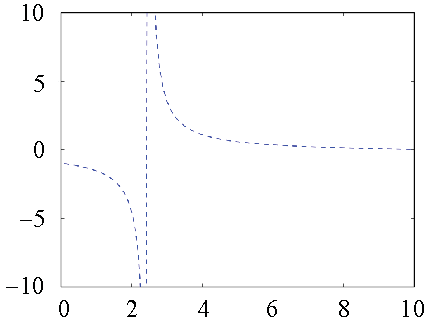
\includegraphics[width=7cm]{./figures/TwoAtF1.pdf}
\caption{$a_s$ 和 $V_0$ 的关系} \label{TwoAtF_fig1}
\end{figure}

大致如\autoref{TwoAtF_fig1},横坐标 $V_0$,纵坐标 $a_s$. 可以看到,$a_s$ 会迅速的变成负无穷,然后再变成正无穷.

当然这是一个针对我们已经知道势能形式的验证;如果想要得到一些实验上可以测量的东西的话,就是
\begin{equation}
\dv{\sigma}{\Omega} = \frac{1}{k^2}\Big|\sum_{l=0}^{+\infty}  (2l+1) \frac{\E^{\I\delta_{lk}}\sin\delta_{lk}}{k} P_l(\cos\theta) \Big|^2
\end{equation}

之前说的时候我们注意到这个 $r_0$ 是很重要的一个假设;但是如果我们有一个长程力会发生什么呢?实际上,有人证明,如果力的作用是 $r^{-\alpha}$ 的形式,那么对于 $l$ 波,
\begin{equation}
\begin{split}
\tan\delta_k \propto k^{2l+1} &(2l+1\le\alpha-2)\\
\tan\delta_k \propto k^{\alpha - 2} &(2l+1\ge\alpha-2)
\end{split}
\end{equation}

提一句, $l$ 越高,$\delta_k$ 与 $k$ 的关系幂次越高,所以相移就 $\to 0$,表明几乎没有相互作用.
而我们处理的 $s$ 波问题,要求 $\alpha>3$. van der waals相互作用是 $ar^{-5}+br^{-11}$ 的,显然满足要求.

如果仔细的考虑分波问题的话,把入射的平面波分解展开成球面波,下面式子的左边应该等于右边
\begin{equation}\ali{
&f(\theta)\frac{\E^{\I kr}}{r} + \frac{1}{2\I kr}\left[\sum_{l=0}^{+\infty}(2l+1)P_l(\cos\theta)\left(\E^{\I kr}- \E^{-\I(kr-\pi l)}\right)\right] \\
= &\sum_{l=0}^{+\infty}\frac{\chi_{kl}(r)}{kr}P_l(\cos\theta)
}\end{equation}

而可以显然的看到
\begin{equation}\ali{
\E^{\I kr}- \E^{-\I(kr-\pi l)} &= \E^{\I\pi l/2}\left(\E^{\I(kr-\pi l/2)} - \E^{-\I(kr-\pi l/2)}\right)\\
&= \I^l 2\I\sin(kr-\frac{\pi l}{2})
}\end{equation}

其中定义得到的散射成分为
\begin{equation}
f(\theta)\frac{\E^{\I kr}}{r}
\end{equation}

而第二项是平面波 $\E^{\I kz}$ 的拆分. 不妨假设
\begin{equation}
f(\theta) = \sum_{l=0}^{+\infty}D_l P_l(\cos\theta)
\end{equation}

从而,在 $r\to\infty$ 的时候,考虑 $l$ 成分:
\begin{equation}
A_l\sin(kr-\frac{\pi}{2}l + \delta_l) = \I^l (2l+1)\sin(kr-\frac{\pi}{2}l) + k\E^{\I kr}D_l
\end{equation}

而 $D_l$ 是个数,与 $r$ 无关,那么显然我们就有
\begin{equation}
\frac{\partial}{\partial r}\left[\E^{-\I kr}\left(A_l\sin(kr-\frac{\pi}{2}l + \delta_l) - \I^l (2l+1)\sin(kr-\frac{\pi}{2}l)\right)\right] = 0
\end{equation}

从而计算得到
\begin{equation}
f(\theta) = \frac{1}{2\I k}\left[\sum_{l=0}^{+\infty}(2l+1)P_l(\cos\theta)\left(\E^{2\I\delta_l}-1\right)\right]  = 0
\end{equation}

和
\begin{equation}
A_l = \I^l(2l+1)\E^{\I\delta_l}
\end{equation}

对于 $s$ 成分,有
\begin{equation}\ali{
f_s(\theta) &= \frac{\E^{2\I\delta}-1}{2\I k} = \frac{\sin\delta \E^{\I\delta+\pi/2}}{\I k} = \frac{\sin\delta}{k \E^{-\I\delta}} = \frac{\sin\delta}{k(\cos\delta - \I\sin\delta)} \\
&= \frac{1}{-\I k+k/\tan\delta} = \frac{1}{-\I k-1/a_s}
}\end{equation}

可以看出来,当 $ka_s\ll1$ 时, $f_s\sim -a_s$,此时 $s$ 波散射的散射截面 $\sigma = 8\pi |f(\theta)|^2 = 4\pi a_s^2$;而另一个极限, $ka_s\gg1$ 时, $f_s\sim- 1/(\I k)$, $\sigma = 8\pi/k^2$.

注意到,在第二个极限的时候,散射强度只与动能大小相关,我们称之为unitary区域.

就像固体里面一样,我们这里可以定义一个\textbf{赝势}从而得到我们想要的 $a_s$. 具体如何得到呢?我们通过如下这种特殊的势能: $\delta$ 势
\begin{equation}
V(r) = \delta(r)\hat{\mathcal{O}}(r)
\end{equation}

这个势需要满足对于任意的 $\forall r$ 都有统一的薛定谔方程,而且解是我们期望的(低能的)
\begin{equation}
\Psi(r) = \frac{\sin(kr+\delta_k)}{kr}\to \frac{1}{kr} - \frac{1}{ka_s}
\end{equation}

显然,动能部分得到非常简单的结果
\begin{equation}
-\frac{\hbar^2}{2m}\nabla^2\Psi(r) = -\frac{\hbar^2}{2mk}\nabla^2 \frac{1}{r} + -\frac{\hbar^2}{2m}\nabla^2\frac{1}{ka_s} = -\frac{\hbar^2}{2mk}4\pi\delta(r)
\end{equation}

势能为了满足薛定谔方程,应该,
\begin{equation}
\delta(r)\hat{\mathcal{O}}(r)\Psi(r) = \frac{\hbar^2}{2mk}4\pi\delta(r)
\end{equation}

从积分角度理解,有
\begin{equation}
\int\delta(r)\hat{\mathcal{O}}(r)\Psi(r) = \hat{\mathcal{O}}(r)\Psi(r)|_{r=0} =  \hat{\mathcal{O}}(r)\left(\frac{1}{kr} - \frac{1}{ka_s}\right)|_{r=0} \overset{\text{should}}{=} \frac{\hbar^2}{2mk}4\pi
\end{equation}

那么,可以看出,如果我们令

\begin{equation}
\hat{\mathcal{O}}(r) = \frac{\hbar^2}{2m}4\pi a_s \partial_r\cdot r
\end{equation}

其显然有
\begin{equation}
\hat{\mathcal{O}}(r)\frac{1}{kr} = \frac{\hbar^2}{2m}4\pi a_s \partial_r \frac{1}{k} = 0
\end{equation}
\begin{equation}
\hat{\mathcal{O}}(r)\frac{1}{ka_s} = \frac{\hbar^2}{2m}4\pi a_s \partial_r \frac{r}{ka_s} = \frac{\hbar^2}{2mk}4\pi
\end{equation}

也就是说满足我们的要求.

接下来,我们考察另外一种情况:我们考虑点接触势,也就是说 $V(r) = g\delta(r)$. 注意,这里的 $g$ 不应该理解为一个参数. 如果强行理解为一个参数,由于波函数的发散,我们通常这里需要进行\textbf{重整化操作}.

在这种考虑下,相互作用 Hamiltonian 就可以写为
\begin{equation}
\mathcal{H} = \int \text{d}^3{\bvec r}\left(\psi\Her\left(-\frac{\hbar^2}{2m}\nabla^2\right)\psi+g\psi\Her\psi\Her\psi\psi\right)
\end{equation}

我们可以建立两体散射的 $T$ 矩阵,并且只考虑 ladder 图. 如图:

\begin{figure}[ht]
\centering
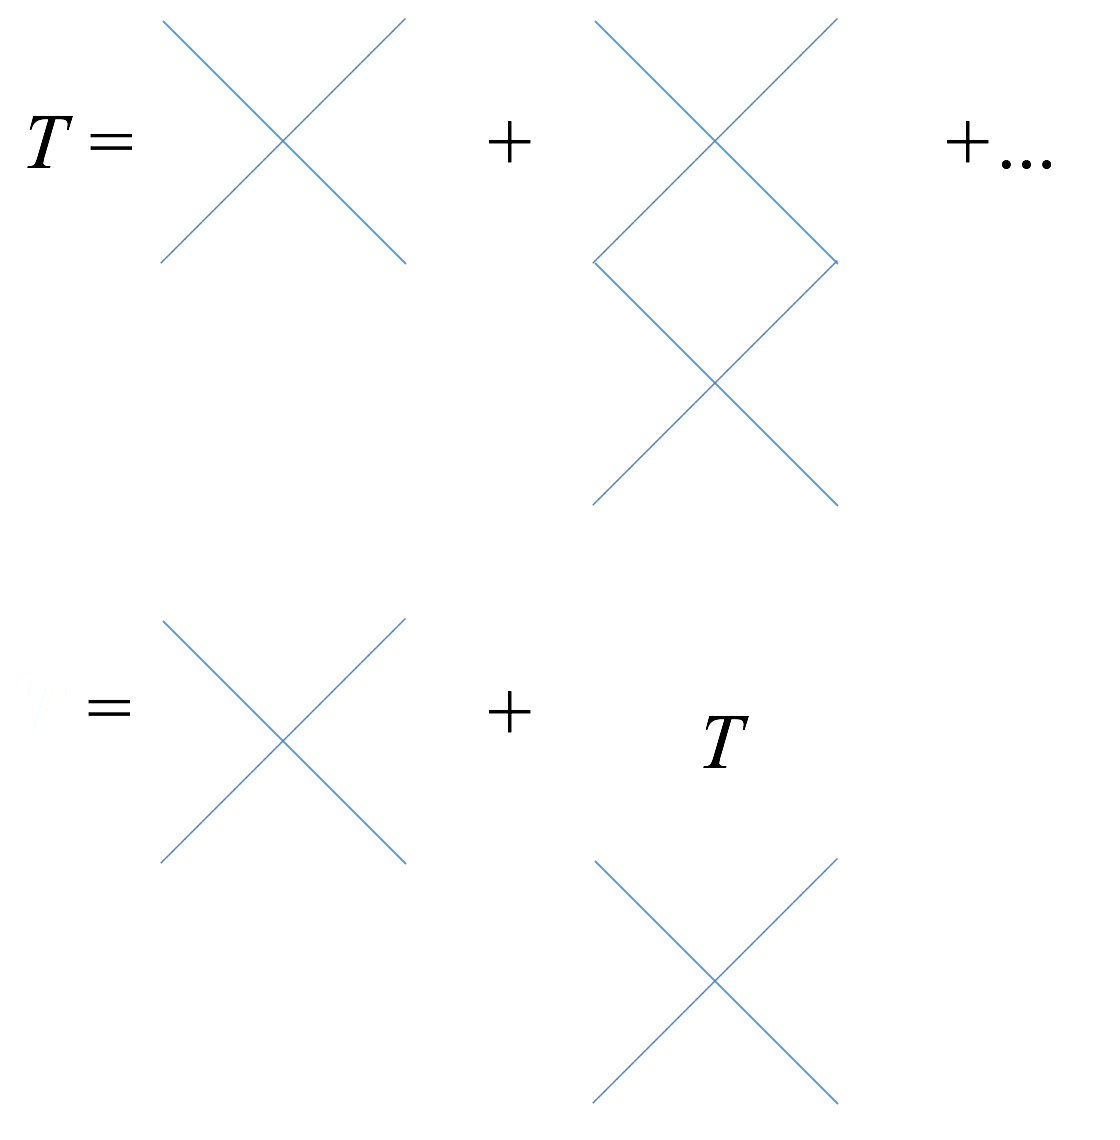
\includegraphics[width=6cm]{./figures/TwoAtF2.png}
\caption{ladder 图} \label{TwoAtF_fig2}
\end{figure}

也就是说我们可以写出形如 $T=g + fT$ 的self-consistant形式.

通过分析知道,最后 $T$ 矩阵实际上是散射的入射能量的函数,也就是说,可以写成 $T(E)$ 的形式,有
\begin{equation}
T(E) = g + \frac{g}{V}\sum_{\bvec k}\frac{1}{E-\hbar^2{\bvec k}^2/m}T(E)
\end{equation}
其中第二项包含一个顶角、可供交换的动量 ${\bvec k}$ 以及相应带来的传播子. 形式上我们解得
\begin{equation}\ali{
T(E) &= \dfrac{g}{1 -  \frac{g}{V}\sum_{\bvec k}\frac{1}{E-\hbar^2{\bvec k}^2/m}}\\
&= \dfrac{1}{\frac{1}{g} + \frac{1}{V}\sum_{\bvec k}\frac{1}{\hbar^2{\bvec k}^2/m} -  \frac{1}{V}\sum_{\bvec k}\left(\frac{1}{E-\hbar^2{\bvec k}^2/m} + \frac{1}{\hbar^2{\bvec k}^2/m}\right)}
}\end{equation}
分母的第三项可以计算:
\begin{equation}
\begin{split}
&\frac{1}{V}\sum_{\bvec k}\left(\frac{1}{E-\hbar^2{\bvec k}^2/m} + \frac{1}{\hbar^2{\bvec k}^2/m}\right)\\
=&\frac{mE}{V\hbar^2}\sum_{\bvec k}\frac{1}{{\bvec k}^2(E-\hbar^2{\bvec k}^2/m)} 
\end{split}
\end{equation}

求和可以变成积分,补上差的系数并且根据对称性,我们得到
\begin{equation}
\begin{split}
=&\frac{V}{(2\pi)^3}\frac{1}{V}\int\text{d}^3{\bvec k}\left(\frac{1}{E-\hbar^2{\bvec k}^2/m} + \frac{1}{\hbar^2{\bvec k}^2/m}\right)\\
=&\frac{m}{2\pi\hbar^2}\int\text{d}k\frac{1}{1-\hbar^2k^2/mE} 
\end{split}
\end{equation}

令 $k_0 = \sqrt{mE/\hbar^2}$,结合留数定理(注意这里是奇点在实轴上,我们只有主值)我们有
\begin{equation}
\begin{split}
=&\frac{m}{2\pi\hbar^2}\int\text{d}k\frac{1}{1-k^2/k_0^2} \\
=&\frac{m}{2\pi\hbar^2}\cdot 2\cdot \pi \I \cdot \left(-\frac{k_0}{2}\right)\\
=&\frac{-\I mk_0}{2\pi\hbar^2}
\end{split}
\end{equation}

于是
\begin{equation}
T(E) = \dfrac{1}{\frac{1}{g} + \frac{1}{V}\sum_{\bvec k}\frac{1}{\hbar^2{\bvec k}^2/m} + \frac{\I mk_0}{2\pi\hbar^2}}
\end{equation}

利用散射振幅与 $T$ 矩阵的关系:
\begin{equation}
T=\frac{4\pi\hbar^2}{m}\frac{1}{1/a_s + \I k} = \dfrac{1}{\frac{1}{g} + \frac{1}{V}\sum_{\bvec k}\frac{1}{\hbar^2{\bvec k}^2/m} + \frac{\I mk_0}{2\pi\hbar^2}}
\end{equation}
实部相等于是我们得到了最重要的一个关系式:
\begin{equation}\label{TwoAtF_eq38}
\frac{ma_s}{4\pi\hbar^2} = \frac{1}{g} + \frac{1}{V}\sum_{\bvec k}\frac{1}{\hbar^2{\bvec k}^2/m}
\end{equation}

对散射相移的一般定义是:散射波函数 $\Psi_{sc}(r) = f(\theta) \E^{\I (kr-\omega t)}/r$ 中的散射振幅 $f(\theta)$ 进行分波展开,
\begin{equation}
f(\theta) = \sum_{l=0}^{+\infty} (2l+1) f_l P_l(\cos\theta)
\end{equation}

得到的 $f_l$ 满足
\begin{equation}
f_l = \frac{\E^{\I\delta_{lk}}\sin\delta_{lk}}{k}
\end{equation}

而在能量很低的时候, $f_l$ 对 $k$ 有一个大概的形式依赖关系:(其中利用了 $j_l(kr)\to a(kr/2)^l$ 以及径向部分 $A_l(r) = \E^{\I\delta_l}[\cos\delta_l j_l(kr) -  \sin\delta_l n_l(kr)]$,在 $\delta\to0$ 时 $A_l(r)\to j_l(kr)$):
\begin{equation}
f_l = -\frac{2m}{\hbar^2}\int_0^{\infty} \dd{r} j_l(kr)V(r)A(r)r^2 \sim k^{2l}
\end{equation}

从而得到在 $k\to0$ 的时候
\begin{equation}
\delta_{lk}\propto k^{2l+1}
\end{equation}
